\chapter{Prototype}\label{ch:proto}

In this third section of my thesis I finally present my self programmed prototype. The State of the Art chapter was structured in such a way, that it focuses on the necessary information for understanding my prototype. Hence I only gave some additional information about techniques which produce even more accurate results, but this is out of scope for my thesis. This section is divided into four sections, starting with the objective (Section \ref{ss:obj}) of this prototype. I propose my requirements for this prototype and what I expect to achieve from it. The next step is the technical concept (Section \ref{ss:tc}), which models the data flows and processes inside the program. After I explain which steps my algorithm goes through, I present snippets of my code in Section \ref{ss:imp} to further illustrate it. This code will be evaluated in Section \ref{ss:eval}.

\section{Objective}\label{ss:obj}

\textit{"I don't have time to read the entire report, please give me a brief summary"}. Many years ago the challenge was to find the right information for a specific tasks, nowadays the internet provides more information than anyone could ever read. Depending on the type of document or article, it is not always necessary to read it from the beginning to the end. Throughout my thesis I often used my case study \textit{News Headline Summarization from Google} for illustrating certain concepts. I chose a different topic for my case study than my actual prototype to show another kind of task which automatic text summarization is capable of.

I chose the \textbf{Amazon Fine Food Reviews} provided from \textit{Stanford Network Analysis Project} hosted on the website Kaggle \footnote{https://www.kaggle.com/snap/amazon-fine-food-reviews/}. This website is commonly known for providing data-sets from private and organizational publishers. 

The project's objective is to build and train a model that can compute relevant summaries for reviews written about fine foods sold on Amazon. 

This dataset contains around 500.000 entries with each entry containing one review from the amazon fine foods and its summary. The data is collected for 8 years from October 2012 until now. 

\section{Technical concept}\label{ss:tc}

An example review needs to pass from the given data-set file to the predicted summary a lot of processes and transformations. The technical concept illustrates all necessary steps without yet going into the programming detail itself. The purpose of this section is to take all the previous explanations into a combined example and show the entire process from the beginning to the end. 

The processing steps follow in chronological order:

\begin{itemize}
	\item Data pre-processing
	\item Build the Model
	\item Train the Model
	\item Generating Summary
\end{itemize}

This steps will be explained in the following Subsection.

\subsection{Data Pre-processing}\label{ss:preprop}

The computer does not understand words. It is not possible to feed the words from a review subsequently into a recurrent neural network and expect that the algorithm will learn it somehow. Performing pre-processing is a crucial step before feeding inputs into the neural network model. The data must be normalized into a clean and not messy way. The following is an example from the original dataset:

\begin{tcolorbox}
	\textbf{Review} \\
	I can remember buying this candy as a kid and the quality hasn't dropped in all these years. Still a superb product you won't be disappointed with. \\
	
	\textbf{Summary} \\
	Delicious product!
\end{tcolorbox}

For all the words occurring in the review and summary a vocabulary dictionary needs to be created. This dictionary can be used to convert the words into numbers and respectively numbers is what the recurrent neural network wants as an input. For creating the two vocabulary dictionaries it needs to be carefully though of how to handle the data. If the same word e.g. \textit{Still} and \text{still} is once with a capital letter and the second time without, the encoding (\textit{UTF-8}) is different and hence the computer regards this as two different words. Furthermore the text can include punctuation, quotation marks or parenthesis. Therefore I defined a chronological order of text transformation steps to normalize the text:

\begin{tcolorbox}
	\begin{itemize}
		\item Convert all words into lowercase
		\item Remove occurring HTML tags
		\item Contraction mapping
		\item Remove (‘s)
		\item Remove any text inside the parenthesis ( )
		\item Eliminate punctuations and special characters
		\item Remove stopwords
		\item Remove short words
	\end{itemize}
\end{tcolorbox}

\textbf{Contraction mapping} describes the process of mapping contracted words into their original two words. For example \textit{haven't} will be mapped back to \textit{have not}. This is important, because only this way the algorithm can detect the word \textit{not} to be negative connotated. If a review says something is not bad, then the algorithm can summarize it by computing the word good. This relation can only be learned by the algorithm by providing it all the necessary words.

\textbf{Remove stopwords} limits the vocabulary size, which reduces the models training time dramatically. I have already explained stopwords in Section \ref{ss:sd}. Those are words like and, that or there. 

\textbf{Remove short words}, because they most likely don't play a vital role in predicting the output. Words like it, in or at not necessarily appear in the stoowords dictionary. For this reason I remove them manually, because they almost don't affect the text's meaning, but after removing the reduce the training time further. 

After applying all of the pre-processing steps, the example will look as the following:

\begin{tcolorbox}
	\textbf{Cleaned Review} \\
	remember buying candy kid quality dropped years still superb product disappointed \\
	
	\textbf{Cleaned Summary} \\
	delicious product
\end{tcolorbox}

The data is now clean and normalized. Furthermore it can be check whether some data is duplicated and remove this data respectively. 

\begin{figure}
	\begin{center}
		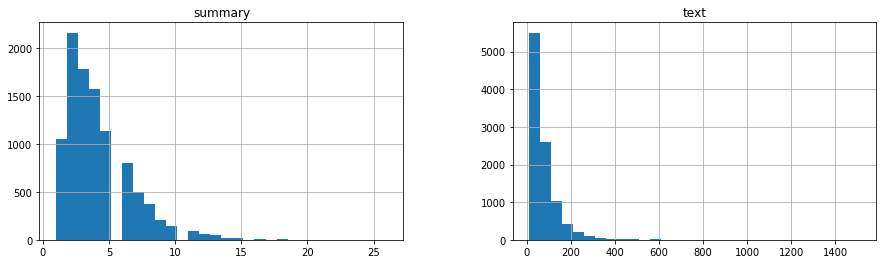
\includegraphics[width=6in]{photos/dist_seq}\\
		\caption{Distribution of the sequences to estimate the maximum length for the review and summary}\label{dist_seq}
	\end{center}
\end{figure}

In order to build the mentioned vocabulary, the text needs to be \textbf{Tokenized}. This means selecting all the single words of a sentence and store all the words uniquely in the vocabulary for the review and the other vocabulary for the summary. The only thing left is to compare the word counts of all sentences and take the median value for the maximum review length and the maximum summary length as shown in Figure \ref{dist_seq}. This is important, because a fixed length is mandatory for building the model. All of the words are now replaced by their dictionary number representation and if a review is shorter as the maximum length, the missing data points are filled with zeros.

\begin{tcolorbox}
	\textbf{Tokenized and Padded Review}
	
	array([[ 678,  142,  360, 1017,   87, 3724,  108,   55, 1893,    9,  243,
	0,    0,    0,    0,    0,    0,    0,    0,    0,    0,    0,
	0,    0,    0,    0,    0,    0,    0,    0,    0,    0,    0,
	0,    0,    0,    0,    0,    0,    0,    0,    0,    0,    0,
	0,    0,    0,    0,    0,    0,    0,    0,    0,    0,    0,
	0,    0,    0,    0,    0,    0,    0,    0,    0,    0,    0,
	0,    0,    0,    0,    0,    0,    0,    0,    0,    0,    0,
	0,    0,    0]], dtype=int32) \\
	
	\textbf{Tokenized and Padded Summary}
	
	array([[ 1, 21, 19,  2,  0,  0,  0,  0,  0,  0]], dtype=int32)
\end{tcolorbox}

This is the necessary format for building up a model.

\subsection{Building the Model}\label{ss:build}

The model follows an abstractive approach (Section \ref{ss:abstractive}) and is based on the Advanced Approaches for Text Generation (Section \ref{ss:aatg}). Since the objective is to build a text summarizer, the input is the fixed length sequence of words and the output is a shorter, but also fixed length sequence of words (Figure \ref{build_model}).
	
The mathematical notations for Figure \ref{build_model} are shown in the box below.
	
\begin{tcolorbox}
	\boldmath{\([x_{1}, x_{2}, x_{3}, ..., {x_{Tx}]}\)} where each \textit{x} represents one word of the input sequence, \\ e.g. \(x_{1}\) = remember \\ \\
	\boldmath{\([y_{1}, y_{2}, x_{3}, ..., {y_{Ty}]}\)} where each \textit{x} represents one word of the input sequence, \\ e.g. \(y_{1}\) = delicious \\ \\
	\boldmath{\(T_{x}\)} represents the fixed length of the input sequence \\ \\
	\boldmath{\(T_{y}\)} represents the fixed length of the output sequence
\end{tcolorbox}

The reason for choosing the LSTM over a basic recurrent neural network architecture is, that the generated summary can be sometimes quite long (up to 20 words) and the recurrent neural network cannot catch up with dependencies of this sequence length. Figure \ref{modelenc} illustrates the overall view of my model. 
As explained in the last section, if a input or output has less words than the maximum length, the missing words are denoted as zero values. This allows the algorithm to not compute any further prediction, because it is a zero multiplication. The encoder decoder architecture is mainly used when the input and output length vary from each other. 

\begin{figure}
	\begin{center}
		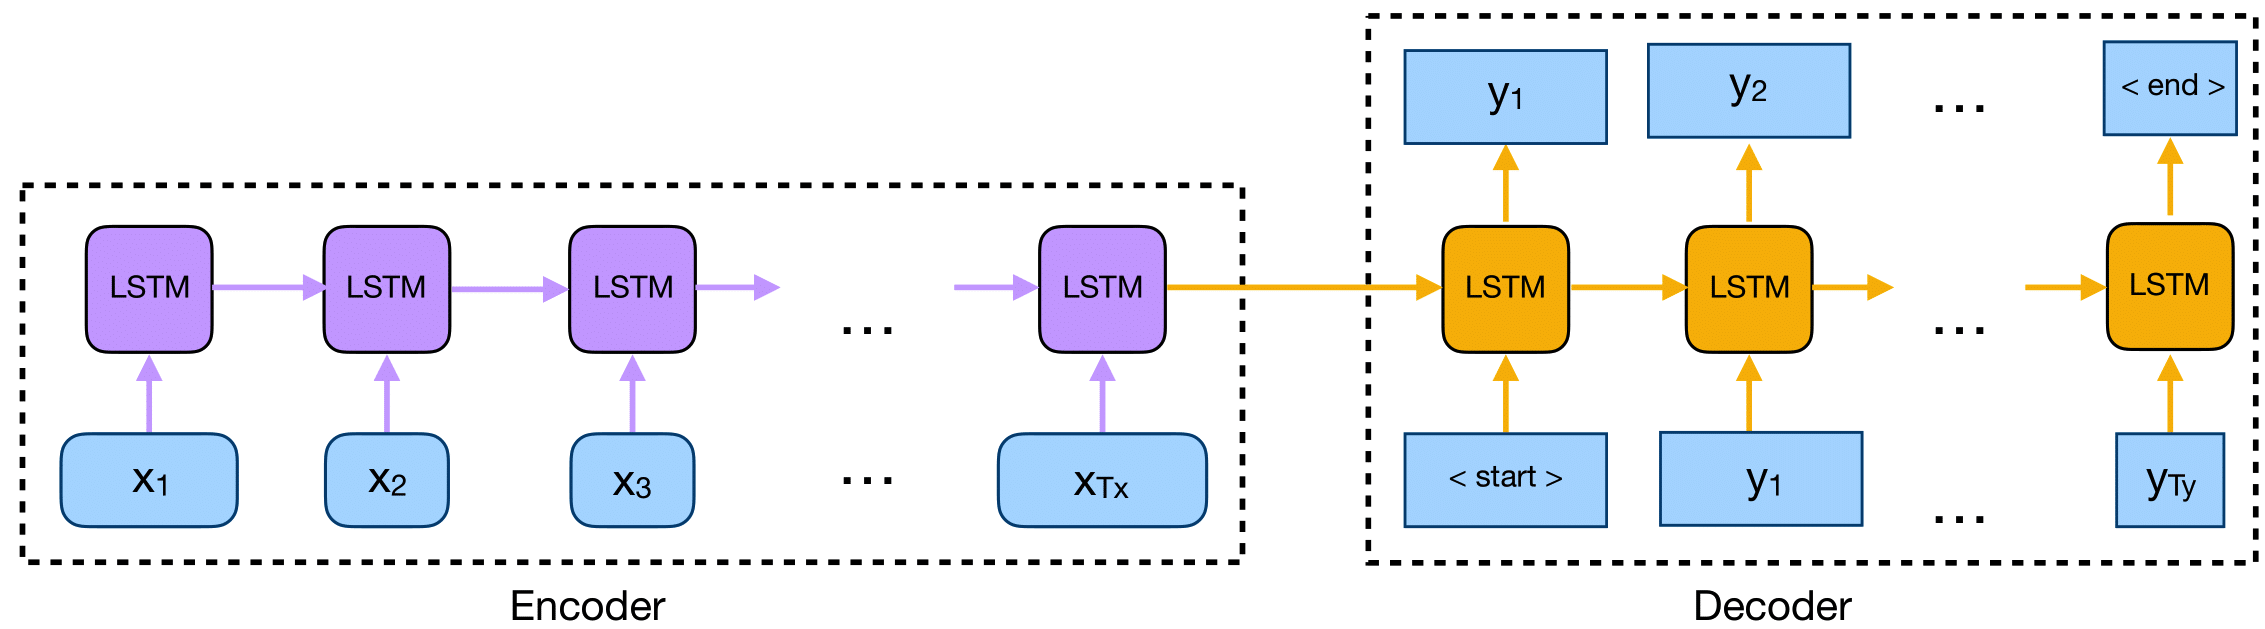
\includegraphics[width=6in]{photos/build-1}\\
		\caption{Many to many Sequence to Sequence LSTM model}\label{build_model}
	\end{center}
\end{figure}

Figure \ref{build_model} shows the general sequence to sequence model, whereas Figure \ref{modelenc} illustrates the perspective of the text summarizer. 

\begin{figure}
	\begin{center}
		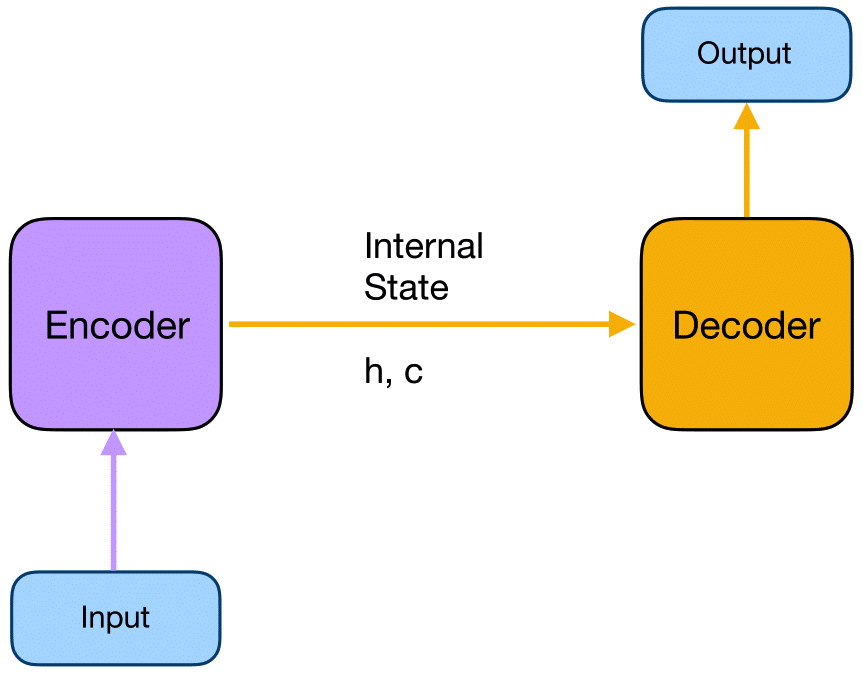
\includegraphics[width=3.5in]{photos/modelenc-1}\\
		\caption{Perspective of the text summarization}\label{modelenc}
	\end{center}
\end{figure}

The mathematical notations for Figure \ref{modelenc} are shown in the box below.

\begin{tcolorbox}
	\boldmath{\(h\)} represents the input (update) gate, which is responsible for adding new information into the cell \\ \\
	\boldmath{\(c\)} represents the cell state, which is the horizontal line between multiple LSTM cells
\end{tcolorbox}

\subsection{Training the Model}

For the training phase, first of all the encoder and decoder need to be set up individually from each other. The model predicts the next word based on the current word (or the start). To achieve this, the prediction is one time step in the future. 

The \textbf{Encoder} in Figure \ref{trainenc} uses LSTM cells to read all of the sentences from the data-set in. Each sentence will be read in at a time and further each word of the sentence will be read for each at a time step. Therefore the LSTM has a one word input per time step and captures the contextual information of the sentence out of it.  The \textit{h} and \textit{c} in Figure \ref{trainenc} are the same as the ones from the previous Figure \ref{modelenc}. 

\begin{figure}
	\begin{center}
		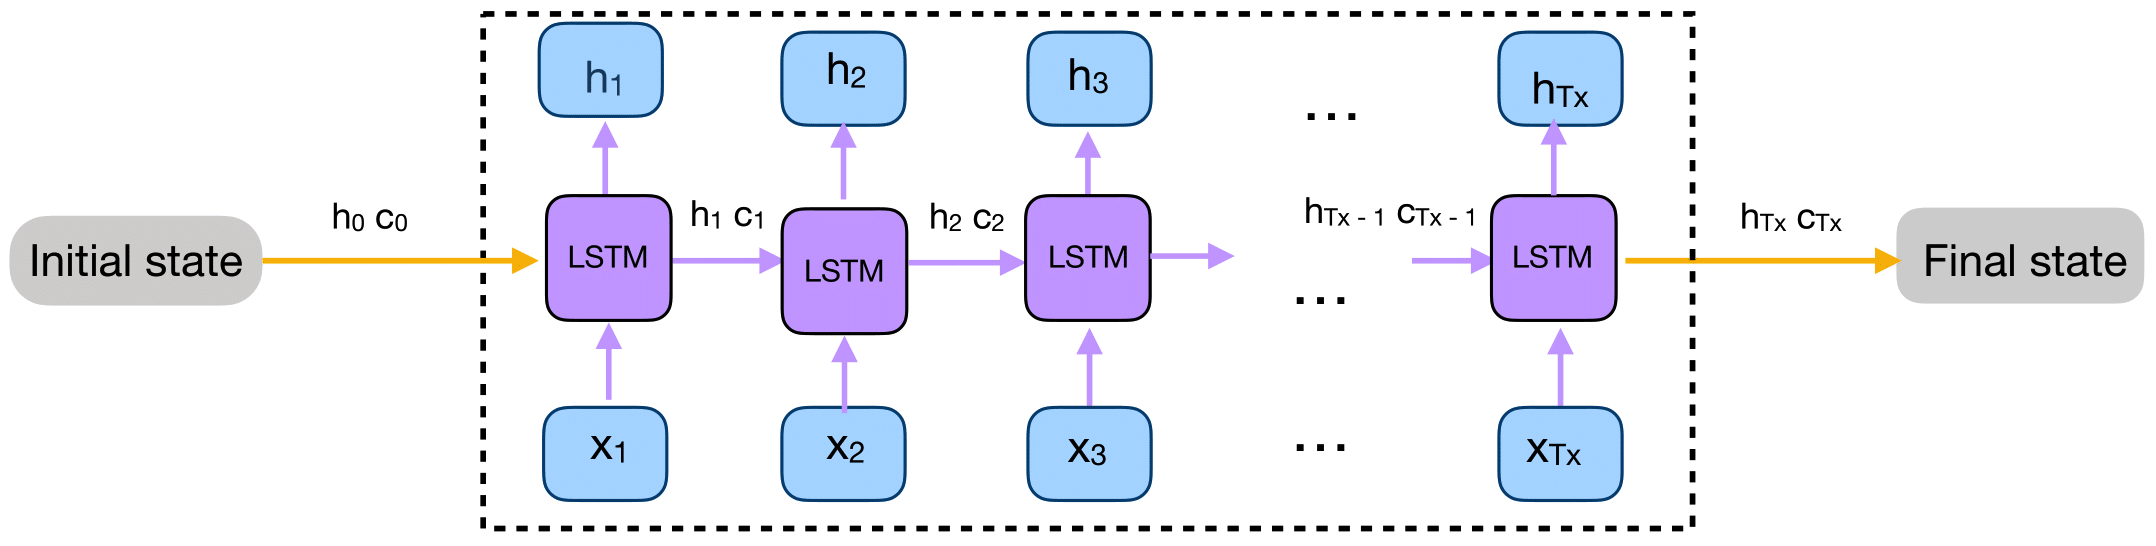
\includegraphics[width=6in]{photos/trainenc-1}\\
		\caption{Encoder of the LSTM}\label{trainenc}
	\end{center}
\end{figure}

The encoder and the decoder are two different LSTM architectures. The initial state of the encoder LSTM is a zero matrix and the finally computed output state of the encoder LSTM is the initial state of the decoder LSTM.

The \textbf{Decoder} is based on a LSTM network as well, which has the target sequence as a word-by-word input and predicts the same sequence offset by one time step. The decoder is trained to predict the upcoming word in the sequence with respect to the previous word. The \textit{start} and \textit{end} boxes in Figure \ref{traindec} represent an appended string to the beginning and ending of the original summary. This is done to create the one time step offset.

\begin{figure}
	\begin{center}
		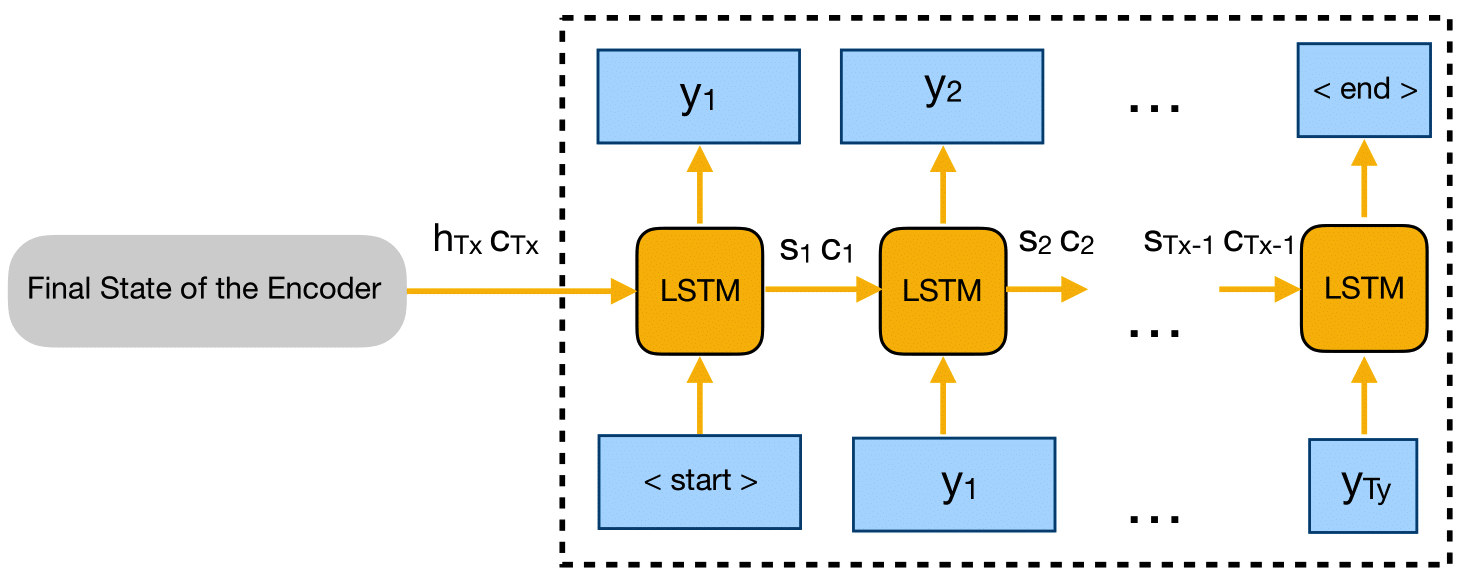
\includegraphics[width=6in]{photos/traindec-1}\\
		\caption{Decoder of the LSTM}\label{traindec}
	\end{center}
\end{figure}

The target sequence is unknown during the decoding part of the test sequence. Target sequence is predicted by passing the first word into the decoder which would is always the \textit{start} token. And the \textit{end} token signals the end of the sentence, followed by potentially zero values.


\subsection{Generate the Summary}\label{ss:generate}

This part is also known as the \textit{Inference Phase}. After training on a selected amount of reviews and summaries, the model is tested on new source sequences where the target sequence is unknown. For this to work,  a inference architecture to decode a test sequence is necessary. The inference goes through various processes:

\begin{itemize}
	\item 1) Encode the review and initialize the decoder with internal states of the encoder
	\item 2) Pass the \textit{start} token as an input to the decoder
	\item 3) Compute the decoder for one time step with the stored internal states
	\item 4) The output at each time step is the probability for the next word. The maximum probability word will be selected
	\item 5) Pass the selected word as an input to the next decoder time step and update the internal states with the current time step
	\item 6) Repeat steps \textit{3} – \textit{5} until the \textit{end} token is generated with the highest probability
\end{itemize}

Figure \ref{infer} shows the architecture for the inference phase. The test sentence goes through all the initially trained weights (states h, c) of the model. There is no more training necessary, just the calculations of the test sequence with the internal state vectors to predict the output sequence. After a certain prediction length, the probability for the \textit{end} token to occur is the highest and if there is remaining space for maximum summary length, it will be filled up with zero values again. 

\begin{figure}
	\begin{center}
		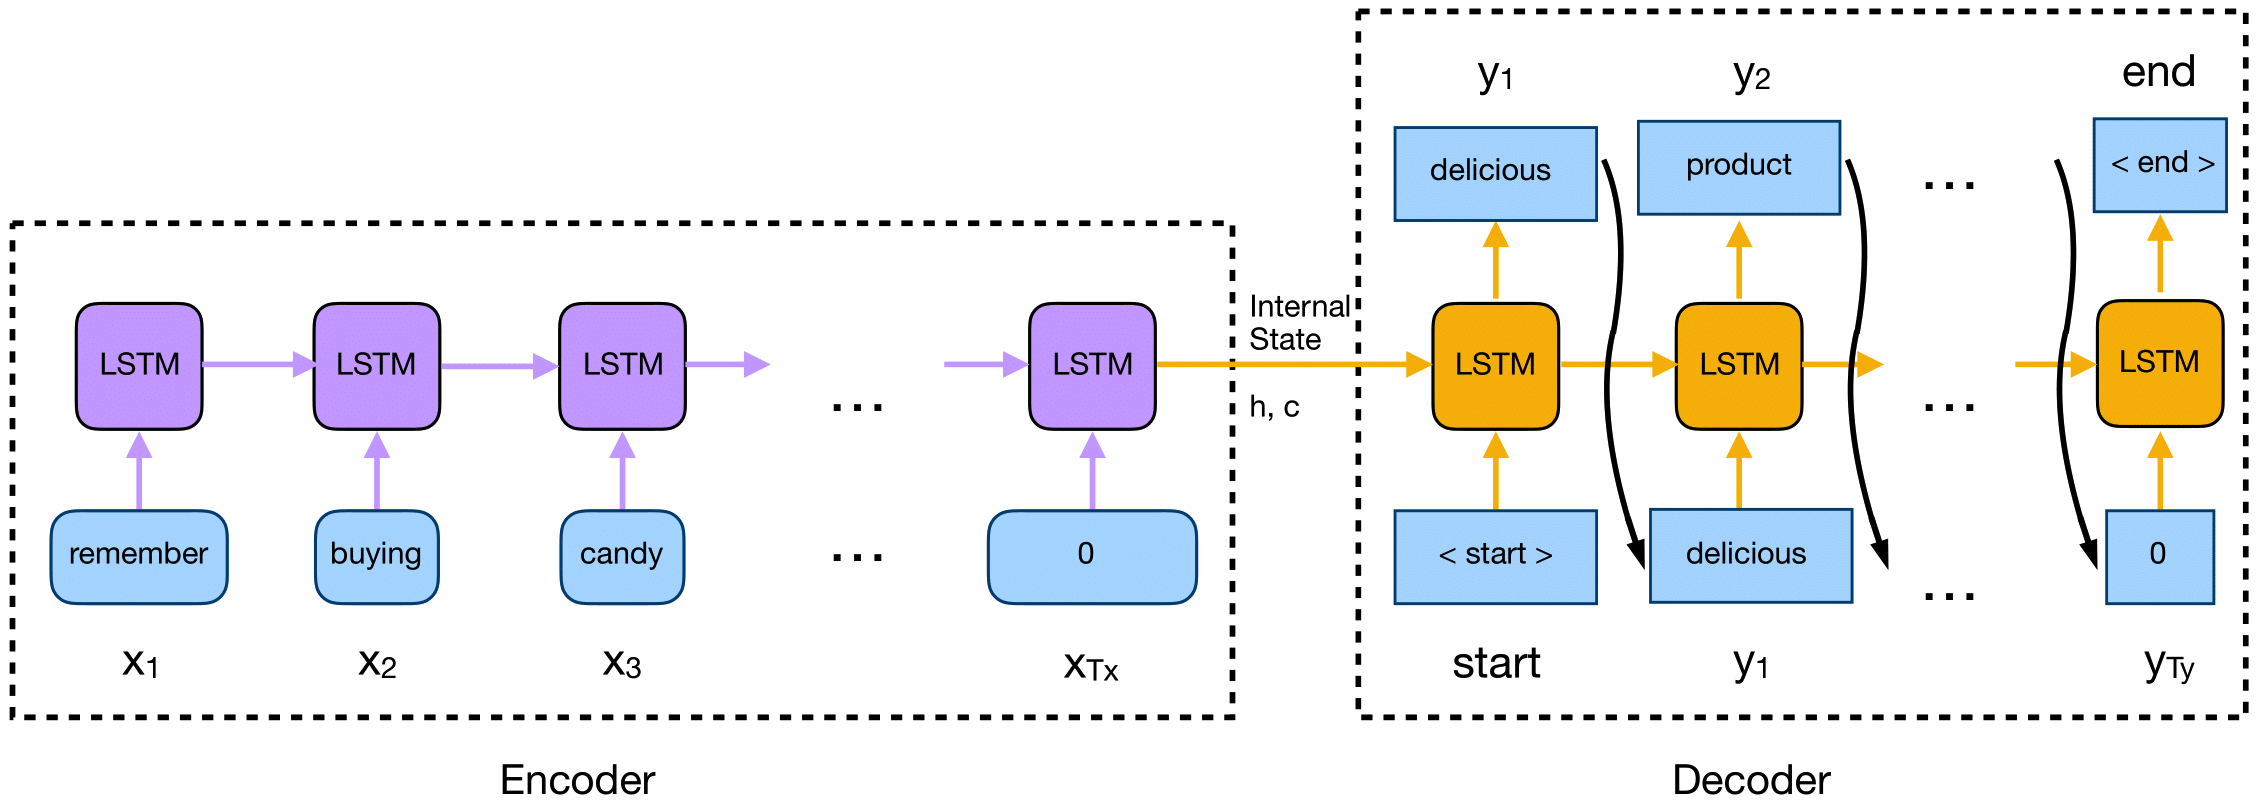
\includegraphics[width=5in]{photos/infer-1}\\
		\caption{Inference architecture to decode a sequence}\label{infer}
	\end{center}
\end{figure}

Even a LSTM cell has limitations when it comes to sentence length. Since summaries can be quite long (my maximum length is 80 words), there need to be made further improvements for the algorithm in order to work properly. It is difficult for the encoder to memorize long sequences and output a fixed length vector. For this reason I have introduced the attention mechanism in Section \ref{ss:atten}. The intuition for attention is:

\begin{tcolorbox}
	\textit{How much attention do we need to pay to every single word in the input sequence for generating a new word at time step \textbf{t}? That is the primal intuition behind the attention mechanism.}
\end{tcolorbox}

With this mechanism it is possible for the decoder to first look on all the words from the encoder output and decide to which parts of the sentence the decoder wants to focus time-by-time. The attention model is placed on top of the LSTM cell and requires additional computation. For my model I am using the \textbf{global attention model} from \cite{effectiveattn} shown in Figure \ref{glob}, where \textit{h} denotes the same weights as Figure \ref{modelenc} and \textit{a} is the attention parameter, calculated for every word at every time step \textit{t}.

\begin{tcolorbox}
	\textbf{h} is the hidden state trained on the encoder \\ \\
	\textbf{t} is the time step which represents always a single word \\ \\
	\textbf{a} is calculated \boldmath{\(T_{y}\)} times at every time step \textbf{t}, so for the attention model we have \textbf{a} * \boldmath{\(T_{y}\)} * \textbf{t} new parameters
\end{tcolorbox}

\begin{figure}
	\begin{center}
		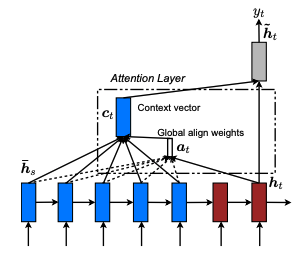
\includegraphics[width=3.5in]{photos/glob_att}\\
		\caption{Global Attention Model from \cite{effectiveattn}}\label{glob}
	\end{center}
\end{figure}

\section{Implementation}\label{ss:imp}

I will not provide the entire code in this section, but I will introduce the most crucial aspects of the code. I used python version 3.7.6 and I programmed it entirely in the \textbf{Anaconda}\footnote{https://www.anaconda.com/} IDE (Integrated Development Environment). This IDE makes it especially easy for programming data science related topics like text summarization in python, because it can preview each cell one-by-one. Anaconda is for free and a open source platform. The python packages I used for this project are listed in the following Listing:

\begin{python}
import numpy as np  
import pandas as pd 
import re           
from bs4 import BeautifulSoup 
from keras.preprocessing.text import Tokenizer 
from keras.preprocessing.sequence import pad_sequences
from nltk.corpus import stopwords   
from tensorflow.keras.layers import Input, LSTM, Embedding, Dense, Concatenate, TimeDistributed
from tensorflow.keras.models import Model
from tensorflow.keras.callbacks import EarlyStopping
\end{python}

\textbf{Numpy} takes care of the computations and data structures. This package is implemented in such a efficient and effective way, so that it saves up a lot of computation time when using this package instead of the default python data structures and mathematical operations.

\textbf{Pandas} is responsible for most of the data pre-processing. The amazon reviews are loaded into a so called Pandas \textit{DataFrame}. Within the DataFrame the data goes through all the necessary pre-processing steps as explained in Section \ref{ss:preprop}. Within the pre-processing step \textit{Remove occurring HTML tags}, the package \textbf{BeautifulSoup} is a useful tool for achieving this step. \textbf{NLTK} is short for Natural Language Toolkit. Many functions regarding Natural Language Processing can be used from this package, but I used it only for downloading the \textit{stopword} for the second last pre-processing step \textit{Remove stopwords}.

\textbf{Keras} is the main package for building the model in Section \ref{build_model}. Keras is built up from the package \textbf{Tensorflow}. TensorFlow has a high-level API for building and training deep learning models. It can be used for doing fast prototyping or state of the art research \footnote{https://www.tensorflow.org/guide/keras}. Since the new update from Tensorflow version 1 to version 2, Keras is normally integrated into the project with Tensorflow (tensorflow.keras indicates Keras is downloaded within Tensorflow). Keras includes most of the required building blocks, such as the LSTM cell or the Embedding Layer which is responsible for mapping the words into vectors. In the following is the encoder part of the trainable model: \\ \\ \\ \\ \\ \\ \\ \\


\begin{python}[caption={Encoder in Python}]
# Encoder 
encoder_inputs = Input(shape=(max_len_text,)) 
enc_emb = Embedding(x_voc_size, latent_dim,trainable = True)
(encoder_inputs) 

#LSTM 1 
encoder_lstm1 = LSTM(latent_dim,return_sequences = True, return_state=True) 
encoder_output1, state_h1, state_c1 = encoder_lstm1(enc_emb) 

#LSTM 2 
encoder_lstm2 = LSTM(latent_dim,return_sequences = True, return_state=True) 
encoder_output2, state_h2, state_c2 = encoder_lstm2
(encoder_output1) 

#LSTM 3 
encoder_lstm3  =LSTM(latent_dim, return_state=True, 
return_sequences = True) 
encoder_outputs, state_h, state_c = encoder_lstm3(encoder_output2) 
\end{python}

The encoder is initialized with the mentioned maximum length of the summary. The Embedding layer creates the vectors out of the input reviews with the limitation of the maximum unique vocabulary word length. The \textit{latent\_dim} parameter denotes the amount of units used for the embedding, in my case I used a value of 500. The encoder is further built up from three LSTM building blocks which is called a \textit{Stacked LSTM}, that has multiple layers of LSTM's stacked on top of each other. This can lead to a better representation of the sequence. The two used parameters for the LSTM are explained in the following:

\begin{itemize}
	\item \textbf{Return Sequences = True}: When the return sequences parameter is \textit{True}, the LSTM produces the hidden state \textit{h} and cell state \textit{c} for every time step
	\item \textbf{Return State = True}: When the return state = \textit{True}, the LSTM produces the hidden state \textit{h} and cell state \textit{c} only from last time step 
\end{itemize}

Those parameters are used the same way for the decoder part of the model. The decoder takes, as explained, the output of the encoder as input into its model. The decoder uses a single LSTM block and also the Attention building block. The only difference is that the attention block is not officially support by Tensorflow, hence it needs to be important through a third-party library or important through an extensible python file. For my model I am using the Bahdanau attention implementation introduced in the paper \textit{Neural machine translation by jointly learning to align and translate} \cite{bah}.

The output of the decoder is fed into the \textit{TimeDistributed} layer, which creates the time steps \textit{t}. The attention layer is concatenated with the decoder layer and the defined model at the end of the following code combines the encoder, attention and the decoder together: \\ \\ \\

\begin{python}
# Decoder. 
decoder_inputs = Input(shape = (None,)) 
dec_emb_layer = Embedding(y_voc_size, latent_dim, trainable=True) 
dec_emb = dec_emb_layer(decoder_inputs) 

#LSTM using encoder_states as initial state
decoder_lstm = LSTM(latent_dim, return_sequences = True, return_state=True) 
decoder_outputs,decoder_fwd_state, decoder_back_state = decoder_lstm(dec_emb, initial_state = [state_h, state_c]) 

#Attention Layer
attn_layer = AttentionLayer(name='attention_layer') 
attn_out, attn_states = attn_layer([encoder_outputs, decoder_outputs]) 

# Concat attention output and decoder LSTM output 
decoder_concat_input = Concatenate(axis=-1, name='concat_layer')([decoder_outputs, attn_out])

#Dense layer
decoder_dense = TimeDistributed(Dense(y_voc_size, activation='softmax')) 
decoder_outputs = decoder_dense(decoder_concat_input) 

# Define the model
model = Model([encoder_inputs, decoder_inputs], decoder_outputs) 
\end{python}

The summarized model looks now like Figure \ref{model_sum} with its 81.380.367 parameters.

\begin{figure}
	\begin{center}
		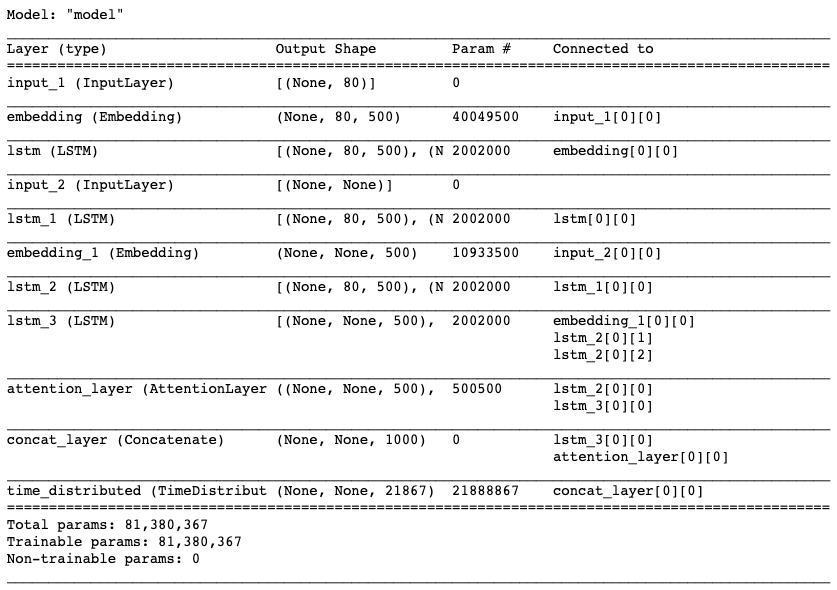
\includegraphics[width=6in]{photos/model_sum}\\
		\caption{Model summarization with parameters}\label{model_sum}
	\end{center}
\end{figure}

\section{Evaluation}\label{ss:eval}

The model and output can be evaluated on multiple ways as explained in Section \ref{ss:ev}. A common approach for evaluating a model is by saving the training and testing loss during each training epoch. The loss function used for this model is the \textit{sparse\_categorical\_crossentropy}, because it converts the integer sequences to a one-hot encoded vector. This prevents a lot of memory issue related problems. One-hot encoding transform arrays into only ones and zeros. The stored losses of each epoch can be plotted into a graph shown in Figure \ref{eval}.

\textbf{Loss}

\begin{figure}
	\begin{center}
		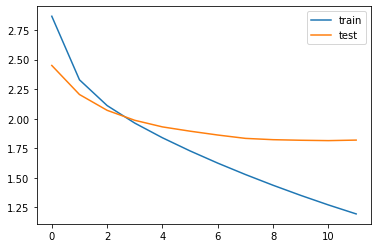
\includegraphics[width=3.5in]{photos/eval}\\
		\caption{Training and validation loss during the training phase}\label{eval}
	\end{center}
\end{figure}

Figure \ref{eval} shows, that the training can be stopped at epoch 10, because the loss is beginning to increase again, which is bad, because the loss needs to be as small as possible. 

Keras provides a prediction function for the model which can be used for a review to generate the summary. The output of the prediction is an integer array which can be mapped back into the original, but cleaned words. The following table presents the computed summaries with the input reviews and the original summaries as a check for quality of the summaries:

\textbf{Predictions}

\begin{table}[]
	\begin{tabular}{@{}cccl@{}}
		\toprule
		\textbf{Cleaned Review}                                                                                                                                                           & \textbf{Cleaned Summary}                                                                   & \multicolumn{1}{l}{\textbf{Generated Summary}} &  \\ \midrule
		\multicolumn{1}{|c|}{\begin{tabular}[c]{@{}c@{}}ordered chips found salty \\ dry huge amount spices \\ ball one bags opened\end{tabular}}                                         & \multicolumn{1}{c|}{\begin{tabular}[c]{@{}c@{}}too salty \\ and dry\end{tabular}}          & \multicolumn{1}{c|}{too salty}                 &  \\ \cmidrule(r){1-3}
		\multicolumn{1}{|c|}{\begin{tabular}[c]{@{}c@{}}found tea favorite movie theater\\  found perfect tea guests \\ everyone loves makes love\end{tabular}}                           & \multicolumn{1}{c|}{\begin{tabular}[c]{@{}c@{}}at the movies \\ and home\end{tabular}}     & \multicolumn{1}{c|}{love it}                   &  \\ \cmidrule(r){1-3}
		\multicolumn{1}{|c|}{\begin{tabular}[c]{@{}c@{}}dogs special diet treats\\  feed favorites cause problems\end{tabular}}                                                           & \multicolumn{1}{c|}{must be good}                                                          & \multicolumn{1}{c|}{my dogs love these}        &  \\ \cmidrule(r){1-3}
		\multicolumn{1}{|c|}{\begin{tabular}[c]{@{}c@{}}delicious sherry flavor salad \\ dressing great used marinade\\ give try sweet balsamic \\ tart red wine vinegar\end{tabular}}    & \multicolumn{1}{c|}{\begin{tabular}[c]{@{}c@{}}yummy sweet \\ sherry vinegar\end{tabular}} & \multicolumn{1}{c|}{love these}                &  \\ \cmidrule(r){1-3}
		\multicolumn{1}{|c|}{\begin{tabular}[c]{@{}c@{}}received medium roast receive \\ correct coffee shown picture \\ disappointed suppose\\  ill try lot trouble return\end{tabular}} & \multicolumn{1}{c|}{wrong coffee received}                                                 & \multicolumn{1}{c|}{coffee received}           &  \\ \bottomrule
	\end{tabular} \\ \\
	\caption{\label{tab:pred}This table shows some example outputs for the training data from my trained model} 
\end{table}

The following predictions have been made with a training of 224814 samples and was validated on 24980 samples for the validation (testing) loss. After epoch 12 the training stopped due of early stopping, because the loss increased again instead of further decreasing. 

\textbf{BLEU Score}

As introduced in Section \ref{ss:ev}, there are two main approaches for evaluating the accuracy of the generated summary. The first way is using the BLEU Score, which was initially published for evaluating machine translation generations. The following Table \ref{tab:rouge} evaluates the predicted summaries from Table \ref{tab:pred} with multiple Rouge Scores.


\begin{table}[]
	\begin{tabular}{@{}lcccc@{}}
		\toprule
		\multicolumn{1}{c}{\textbf{Scoring Method}}                                                                                         & \multicolumn{1}{l}{\textbf{Rouge-1}} & \multicolumn{1}{l}{\textbf{Rouge-2}} & \multicolumn{1}{l}{\textbf{Rouge-L}} & \multicolumn{1}{l}{\textbf{Rouge-BE}} \\ \midrule
		\multicolumn{1}{|l|}{\textbf{\begin{tabular}[c]{@{}l@{}}Original: too salty and dry\\ Predicted: too salty\end{tabular}}}           & \multicolumn{1}{c|}{\textit{0.667}}  & \multicolumn{1}{c|}{0}               & \multicolumn{1}{c|}{\textit{0.667}}  & \multicolumn{1}{c|}{0}                \\ \midrule
		\multicolumn{1}{|l|}{\textbf{\begin{tabular}[c]{@{}l@{}}Original: at the movies and home\\ Predicted: love it\end{tabular}}}        & \multicolumn{1}{c|}{0}               & \multicolumn{1}{c|}{0}               & \multicolumn{1}{c|}{0}               & \multicolumn{1}{c|}{0}                \\ \midrule
		\multicolumn{1}{|l|}{\textbf{\begin{tabular}[c]{@{}l@{}}Original: must be good\\ Predicted: my dogs love these\end{tabular}}}       & \multicolumn{1}{c|}{0}               & \multicolumn{1}{c|}{0}               & \multicolumn{1}{c|}{0}               & \multicolumn{1}{c|}{0}                \\ \midrule
		\multicolumn{1}{|l|}{\textbf{\begin{tabular}[c]{@{}l@{}}Original: yummy sweet sherry vinegar\\ Predicted: love these\end{tabular}}} & \multicolumn{1}{c|}{0}               & \multicolumn{1}{c|}{0}               & \multicolumn{1}{c|}{0}               & \multicolumn{1}{c|}{0}                \\ \midrule
		\multicolumn{1}{|l|}{\textbf{\begin{tabular}[c]{@{}l@{}}Original: wrong coffee received\\ Predicted: coffee received\end{tabular}}} & \multicolumn{1}{c|}{\textit{0.8}}    & \multicolumn{1}{c|}{\textit{0.66}}   & \multicolumn{1}{c|}{\textit{0.8}}    & \multicolumn{1}{c|}{\textit{0.66}}    \\ \bottomrule
	\end{tabular}
	\caption{\label{tab:rouge}The generated Sentences evaluated with the Rouge Score}
\end{table}

It can be seen that the Rouge score produces semantically incorrect scores, because it only looks whether the words in the original and predicted summaries are similar. 

For that reason, the prediction 

\begin{tcolorbox}
	Original: "yummy sweet sherry vinegar" \\
	Prediction: "love these"
\end{tcolorbox}

produces a Rouge score of 0, even though there is a semantic similarity. Whereas the summary

\begin{tcolorbox}
	Original: "wrong coffee received" \\
	Prediction: "coffee received"
\end{tcolorbox}

scores really high, even though the summary is incorrect. The The summary model did not capture the dependency of \textbf{wrong}. For this reason I tried evaluating the five summaries with the \textit{BLEU Score} mentioned in Section \ref{ss:ev}.

\textbf{BLEU Score}

In the following Table \ref{tab:bleu}, I calculated up to the \textit{4-gram} BLEU Scores for the predictions in Table \ref{tab:pred}. 
\begin{table}[]
	\begin{tabular}{@{}lcccc@{}}
		\toprule
		\multicolumn{1}{c}{\textbf{Scoring Method}}                                                                                         & \multicolumn{1}{l}{\textbf{1-gram}}    & \multicolumn{1}{l}{\textbf{2-gram}}    & \multicolumn{1}{l}{\textbf{3-gram}} & \multicolumn{1}{l}{\textbf{4-gram}} \\ \midrule
		\multicolumn{1}{|l|}{\textbf{\begin{tabular}[c]{@{}l@{}}Original: too salty and dry\\ Predicted: too salty\end{tabular}}}           & \multicolumn{1}{c|}{\textit{0.367879}} & \multicolumn{1}{c|}{0.367879}          & \multicolumn{1}{c|}{\textit{0}}     & \multicolumn{1}{c|}{0}              \\ \midrule
		\multicolumn{1}{|l|}{\textbf{\begin{tabular}[c]{@{}l@{}}Original: at the movies and home\\ Predicted: love it\end{tabular}}}        & \multicolumn{1}{c|}{0}                 & \multicolumn{1}{c|}{0}                 & \multicolumn{1}{c|}{0}              & \multicolumn{1}{c|}{0}              \\ \midrule
		\multicolumn{1}{|l|}{\textbf{\begin{tabular}[c]{@{}l@{}}Original: must be good\\ Predicted: my dogs love these\end{tabular}}}       & \multicolumn{1}{c|}{0}                 & \multicolumn{1}{c|}{0}                 & \multicolumn{1}{c|}{0}              & \multicolumn{1}{c|}{0}              \\ \midrule
		\multicolumn{1}{|l|}{\textbf{\begin{tabular}[c]{@{}l@{}}Original: yummy sweet sherry vinegar\\ Predicted: love these\end{tabular}}} & \multicolumn{1}{c|}{0}                 & \multicolumn{1}{c|}{0}                 & \multicolumn{1}{c|}{0}              & \multicolumn{1}{c|}{0}              \\ \midrule
		\multicolumn{1}{|l|}{\textbf{\begin{tabular}[c]{@{}l@{}}Original: wrong coffee received\\ Predicted: coffee received\end{tabular}}} & \multicolumn{1}{c|}{\textit{0.606531}} & \multicolumn{1}{c|}{\textit{0.606531}} & \multicolumn{1}{c|}{\textit{0.8}}   & \multicolumn{1}{c|}{\textit{0.66}}  \\ \bottomrule
	\end{tabular}
	\caption{\label{tab:bleu}The generated sentences evaluated with the BLEU Score}
\end{table}

Since the BLEU Score is evaluating the \textit{n-grams} of the texts, it behaves similarly as the Rouge Score. It can even be said that Rouge and BLEU are complementing each other, due of the BLEU measures how much of the words in the generated summary appear in the original summary, whereas the Rouge measure how much of the words in the original summary appear in the generated summary.

Conducting evaluations on extractive text summarizers turns out to be way easier, because the extractive approach picks its weighted important sentences and appends it to the summary. So it uses only the vocabulary from the trained text. The abstractive summarizer showed to be more complex to evaluate properly due to its flexible structure.
A recent paper in 2019 conducted research in how to properly evaluate an abstractive text summarizer. The team of Kryscinski showed that the current evaluation protocol reflects human judgments only in a week way, while it also fails to evaluate critical features, for example factual correctness (semantic correctness) of text summarization \cite{kryscinski-etal-2019-neural}.